\pagenumbering{arabic}%DO NOT REMOVE THIS
\chapter{Introduction}\label{ch:01intro}

One way of speaking about evolution is with regard to the change in frequencies of alleles (variants of genes) in a population over time. In the field of population genetics, the \textit{Hardy-Weinberg principle} states that genetic variation (diversity of gene frequencies) in a population will remain constant from generation to generation in the absence of disturbances \cite{cutter2019primer}. There are five ``Hardy-Weinberg assumptions'' which must hold for this to be true: no mutation, random mating, no gene flow (i.e. no transferring of genetic material from one population to another), infinite population sizes, and no selection. If any of these assumptions does not hold, then this may change the frequencies of alleles in a population, which allows evolution to occur. The mechanisms for evolution, then, are the opposite of these assumptions, namely: mutation, non-random mating, gene flow, finite populations, and natural selection. Pulling at any of these levers has an effect on the genetic variation of a population and thus impacts their genome. 

Several models have been proposed to illustrate the effects on the population of violating these assumptions. The \textit{Moran model}, named after the Australian statistician Patrick Moran, can be used on populations of finite size to model the impact of neutral drift (a mutation spreading through the population which has no impact on fitness), selection, or mutations. In the simplest version of the neutral drift model, for example, a population consists of two types, A and B, and in each generation one individual is randomly chosen to reproduce and another individual is randomly chosen to die. Given a population with $N$ individuals and $i$ individuals of one type ($0 \leq i \leq N$), the transition probabilities from one state to the next (increasing, decreasing, or maintaining the number of one type) can easily be calculated. The model concludes that given enough time, however, the population reaches \textit{``absorbing''} states in which the population is all of one type, either A or B, with a probability of $\frac{i}{N}$ due to all organisms having equal fitness (and thus being equally likely to be selected at random). The impact of genetic drift on bacterial genome size has been investigated extensively by Kuo et al. \cite{kuo2009consequences} who found further evidence that ``evolutionary forces that act on individual genes have profound effects on the overall architecture of bacterial genomes.'' 

As mentioned above, changes to the population size also causes evolution to occur. The American geneticist Michael Lynch argued in a seminal paper, ``The Origins of Genome Complexity,'' that it was largely due to the increase in organism size\textemdash and thus the decrease in effective population size\textemdash that genome complexity increased, both in prokaryotes (e.g. bacteria) and eukaryotes (e.g. humans). This resulted in an increase in the number of genes and the amount of non-coding DNA, which in turn provided a basis for increased complexity. He argues: ``the transitions from prokaryotes to unicellular eukaryotes to multicellular eukaryotes are associated with orders-of-magnitude reductions in population size; by magnifying the power of random genetic drift, reduced population size provides a permissive environment for the proliferation of various genomic features that would otherwise be eliminated by purifying selection'' \cite{Lynch1401}. 

By contrast, reductive evolution is the process of the average genome size of a species shrinking over time, with respect to both the number of base pairs and genes. For example, some species of bacteria have experienced reductive evolution over the course of millions of years, and this reduction in their genome has lead to a loss of genes, certain regulatory abilities, and more. It has also been theorized that reductive evolution may be responsible for the origin of eukaryotic cells, with the ``symbiogenesis'' theory suggesting that prokaryotic cells may have eventually become the organelles inside eukaryotic cells, with many of the prokaryotic genes being lost due to the mutualistic nature of living in the more protected environment of the cell body~\cite{sagan1967origin}. One bacterial species which has exhibited clear tendencies towards reductive evolution is the marine cyanobacteria \textit{Prochlorococcus}, some of whose strains have experienced a reduction of nearly 40\% of their base pairs when compared to larger strains of their closest living relative, \textit{Synechococcus}. Even among strains of Prochlorococcus, the difference between some of the larger and smaller strains is upwards of 38\% \cite{Batut.2014}. Despite being extensively studied, the underlying mechanisms and full impact of reductive evolution are not fully understood and are an area of intense current research. Several competing explanations exist for these mechanisms, from the influence of population size, genetic drift (defined below), or selection \cite{Batut.2014}, which are discussed in Chapter~\ref{ch:02background}.

Although it would provide more conclusive evidence, performing \textit{in vivo} experiments with living organisms is often impractical because of the difficulty or impossibility of reproducing natural environmental conditions in a laboratory. Such experiments are often too costly in terms of both time and resources. As an alternative, \textit{in silico} experimental evolution is one option that can be used to study the conditions under which an organism's genome may become reduced. In this method, organisms and their evolution over thousands or millions of generations are simulated in software. In this manner, one can control and evaluate every aspect of their evolution over time and a full record of their lineage may be maintained and studied, allowing one to go back and closely examine every step of the evolutionary period for a greater understanding of the factors that lead to specific effects on the genome. The in silico tool \textit{Aevol} is one such platform which realistically models bacterial genomes and evolution, allowing one to draw conclusions about their real-world counterparts. In the following thesis, the results of experiments in artificial evolution are presented which aim to identify and evaluate several factors which potentially lead to changes in genome structure and a reduced genome in simulated bacteria using the Aevol platform. 

Among the difficulties of studying reductive evolution with in vivo evolutionary experiments, one of the most difficult obstacles to overcome is the lack of a full ancestral record. This lack of a full phylogeny can make it difficult or impossible to tell exactly when and how a specific event occurred, or a trait evolved or was lost, as illustrated in Figure \ref{fig:phylogeny03} below. 
\begin{figure}[h]
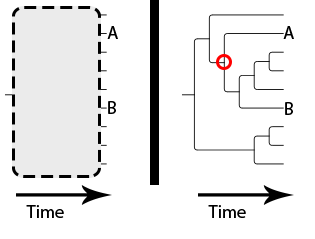
\includegraphics[scale=0.75]{phylogeny03}
\centering
\caption[Unknown phylogeny]{An illustration of unknown phylogeny. Since the phylogenetic information under the shaded box is typically not known, the point of divergence (red circle) can't be determined.}
\label{fig:phylogeny03}
\end{figure}
In this example, two related organisms A and B are compared with an attempt to determine when and how a specific trait was gained or lost by one of the organisms. This may be useful, for example, when attempting to estimate the relative importance (due to conservation over many generations) of some trait. Without the phylogenetic information (under the shaded box) it may not be possible to identify the point in their evolutionary history at which the two organisms diverged, making time estimates difficult or impossible.

Another major downside to in vivo evolutionary experiments is that they are slow. For example, the well-known E. coli Long-Term Evolution Experiment (LTEE) by Profesor Lenski at Michigan State University has been ongoing since February of 1988 and only passed generation 50,000 in 2010, 22 years later\footnote{\url{http://myxo.css.msu.edu/ecoli/celebrate50K.html}}. As an alternative to in vivo experiments, in silico evolutionary experiments are well-suited to the task of studying reductive evolution. Generations of organisms may be evolved within a very short time period, and a full "fossil record" of each lineage may be kept on disk for further analysis. 

The in silico tool Aevol has a realistic artificial chemistry model which was developed specifically to study genome structure. It contains tools to analyze the robustness, fitness, and evolvability of digital organisms over time.  In this thesis, Aevol is used to perform experiments in silico evolution in order to determine the effects of several different conditions on the genome of a simulated ``wild type'' bacteria.

%TODO Hypothesis for reductive genome evolution
%TODO Comparative genomics
%TODO What is interesting about reductive evolution?
%TODO Why is aevol not realistic?
%TODO Are there any other in silico experimental evolution tools?
\section*{Report outline}
%TODO Probably take this out
This chapter serves as the introduction to the thesis and the research problem being faced. In Chapter~\ref{ch:02background}, some necessary background information is provided on reductive evolution, in silico evolution in general, and Aevol in particular. Chapter~\ref{ch:03methods} describes the experimental setup. Chapter~\ref{ch:04results_discussion}
provides the results and analysis of the experiments of this thesis, and Chapter~\ref{ch:05conclusion} presents the conclusions drawn from this work. 


